\documentclass[11  pt]{article} 
\usepackage[lmargin=1in,rmargin=1.75in,bmargin=1in,tmargin=1in]{geometry}  


% For hyperlinking everything
\usepackage{hyperref}
\hypersetup{
	colorlinks=true, %set true if you want colored links
	linktoc=all,     %set to all if you want both sections and subsections linked
	linkcolor=blue,  %choose some color if you want links to stand out
}


\usepackage[latin1]{inputenc}
\usepackage{amsmath}
\usepackage{mathrsfs}  
\usepackage{amsfonts}
\usepackage{amssymb}
\usepackage{graphicx}
\usepackage{subfig}
\usepackage{caption}
\usepackage{algorithm}
%\usepackage{algcompatible}
%\usepackage{algorithmicx}
\usepackage{algpseudocode}

\usepackage{titlesec}
\titleformat{\section}{\fontfamily{lmss}\fontsize{14}{15}\bfseries}{\thesection}{1em}{}
\titleformat{\subsection}{\fontfamily{lmss}\fontsize{12}{15}\bfseries}{\thesubsection}{1em}{}




\usepackage{amsthm}

\newtheoremstyle{noit}
{10pt}% <Space above>
{10pt}% <Space below>
{}% <Body font>
{}% <Indent amount>
{\bfseries}% <Theorem head font>
{.}% <Punctuation after theorem head>
{.5em}% <Space after theorem headi>
{}% <Theorem head spec (can be left empty, meaning `normal')>

\newtheoremstyle{example}
{10pt}% <Space above>
{10pt}% <Space below>
{}% <Body font>
{20pt}% <Indent amount>
{\bfseries}% <Theorem head font>
{.}% <Punctuation after theorem head>
{.5em}% <Space after theorem headi>
{}% <Theorem head spec (can be left empty, meaning `normal')>


\newtheoremstyle{indented}{20pt}{20pt}{\addtolength{\leftskip}{2.5em}}{}{\bfseries}{.}{.5em}{}


\newtheorem{theorem}{Theorem}
\numberwithin{theorem}{section}
\newtheorem{lemma}[theorem]{Lemma}
\newtheorem{corollary}[theorem]{Corollary}
\newtheorem{observation}{Observation}
%\numberwithin{observation}{section}
%\numberwithin{definition}{section}
\newtheorem{conjecture}{Conjecture}
\newtheorem{Qu}{Question}
\newcommand{\QU}{\begin{Qu}\normalfont}

\theoremstyle{noit}
\newtheorem{fact}{Fact}
\newtheorem{definition}{Definition}

\theoremstyle{indented}
\newtheorem{example}{Example}

\theoremstyle{indented}
\newtheorem{problem}{Problem}


%\newenvironment{proof}{\noindent{\bf Proof:} \hspace*{1em}}{
%    \hspace*{\fill} $\Box$ }
%\newenvironment{proof_of}[1]{\noindent {\bf Proof of #1:}
%    \hspace*{1em} }{\hspace*{\fill} $\Box$ }
%\newenvironment{proof_claim}{\begin{quotation} \noindent}{
%    \hspace*{\fill} $\diamond$ \end{quotation}}
\newcommand{\vs}[1]{\vspace{#1}}

\newcommand{\lecture}[2]{
 \noindent
\begin{center}
	\framebox{
		\vbox{
			\hbox to 5.78in { {\bf CSCE 411: Design and Analysis of Algorithms (Honors)} \hfill  }
			\vspace{2mm}
			\hbox to 5.78in { {\Large \hfill Lecture #1\hfill} }
			\vspace{2mm}
			\hbox to 5.78in { {\it Date: #2 \hfill Samson Zhou} }
		}
	}
\end{center}
\vspace*{4mm}
}

\newcommand{\week}[2]{
 \noindent
\begin{center}
	\framebox{
		\vbox{
			\hbox to 5.78in { {\bf CSCE 411: Design and Analysis of Algorithms (Honors)} \hfill  }
			\vspace{2mm}
			\hbox to 5.78in { {\Large \hfill Week #1\hfill} }
			\vspace{2mm}
			\hbox to 5.78in { {\it Date: #2 \hfill Nate Veldt, updated by Samson Zhou} }
		}
	}
\end{center}
\vspace*{4mm}
}

\newcommand{\sweek}[2]{
 \noindent
\begin{center}
	\framebox{
		\vbox{
			\hbox to 5.78in { {\bf CSCE 411: Design and Analysis of Algorithms (Honors)} \hfill  }
			\vspace{2mm}
			\hbox to 5.78in { {\Large \hfill Week #1\hfill} }
			\vspace{2mm}
			\hbox to 5.78in { {\it Date: #2 \hfill Samson Zhou} }
		}
	}
\end{center}
\vspace*{4mm}
}

\newcommand{\hw}[2]{
	\noindent
	\begin{center}
		\framebox{
			\vbox{
				\hbox to 5.78in { {\bf CSCE 411: Design and Analysis of Algorithms} \hfill  }
				\vspace{2mm}
				\hbox to 5.78in { {\Large \hfill Homework #1\hfill} }
				\vspace{2mm}
				\hbox to 5.78in { {\it Due date: #2 \hfil} }
			}
		}
	\end{center}
	\vspace*{4mm}
}



\newcommand{\under}[1]{\underline{\hspace{#1}}}
\setlength{\parindent}{0em}

%\usepackage[tagged]{accessibility}

% Graph terms
\newcommand{\vol}{\textbf{vol}}
\newcommand{\cut}{\textbf{cut}}


% Matrices
\newcommand{\mA}{\textbf{A}}
\newcommand{\mB}{\textbf{B}}

% vectors
\newcommand{\ve}{\textbf{e}}
\newcommand{\vx}{\textbf{x}}


% Other
\newcommand{\calN}{\mathcal{N}}

\usepackage{mathtools}
\DeclarePairedDelimiter\ceil{\lceil}{\rceil}
\DeclarePairedDelimiter\floor{\lfloor}{\rfloor}


\newcommand*{\aitem}{ \item[{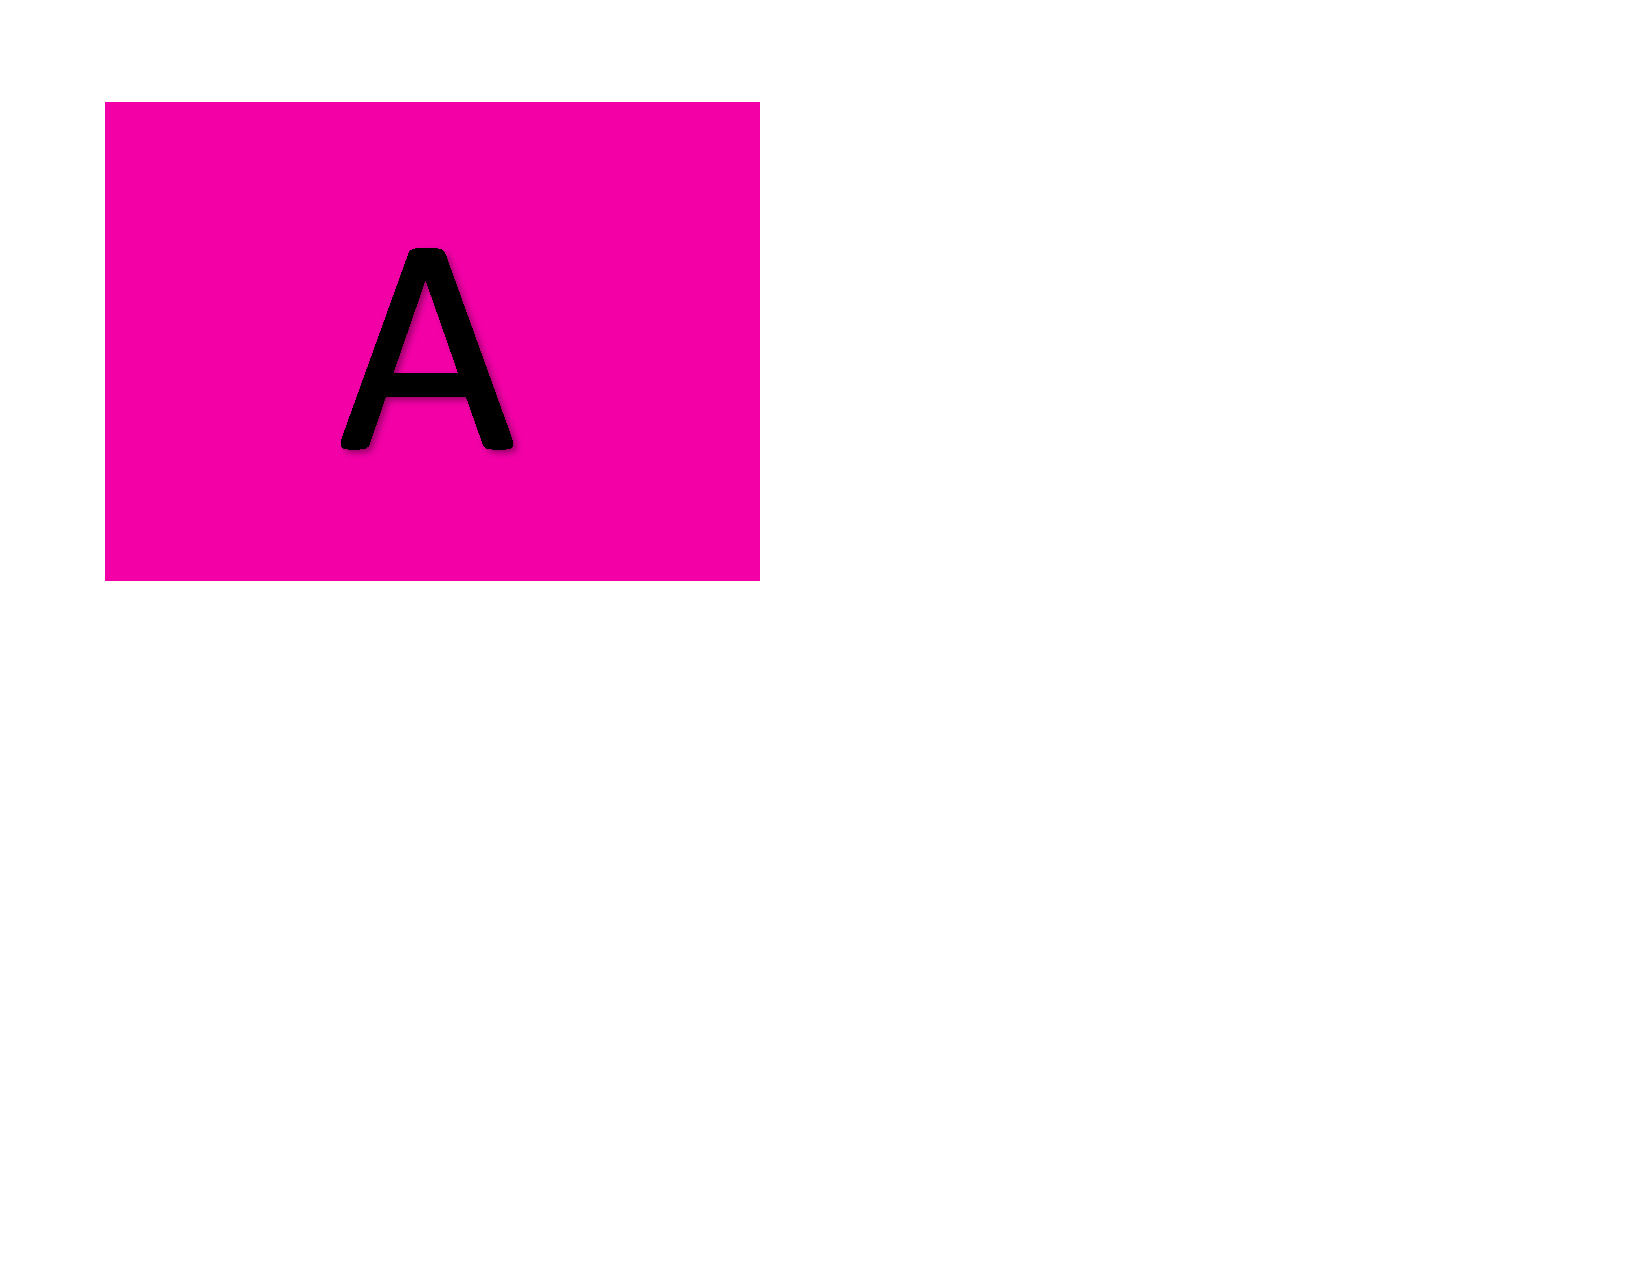
\includegraphics[width=0.8cm,height=0.5cm]{figures/A}} ]  }
\newcommand*{\bitem}{ \item[{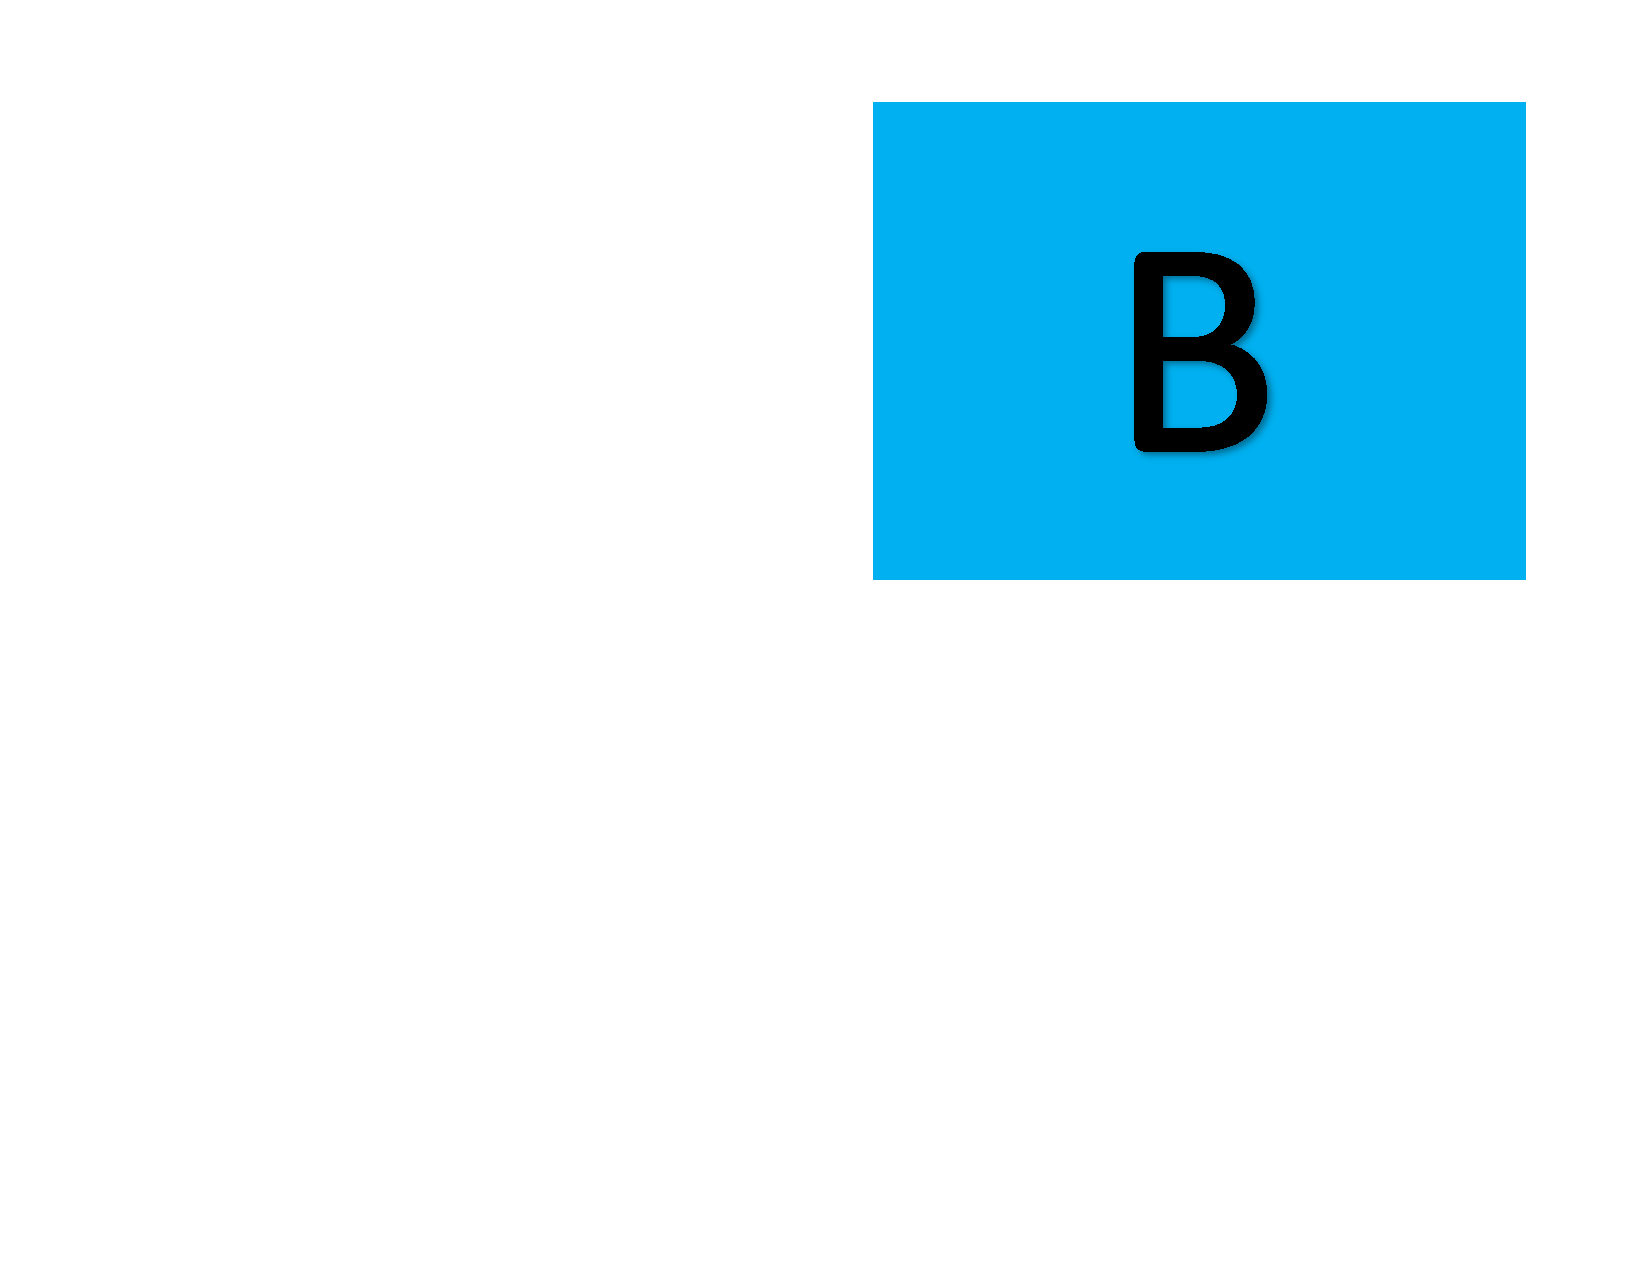
\includegraphics[width=0.8cm,height=0.5cm]{figures/B}} ]  }
\newcommand*{\citem}{ \item[{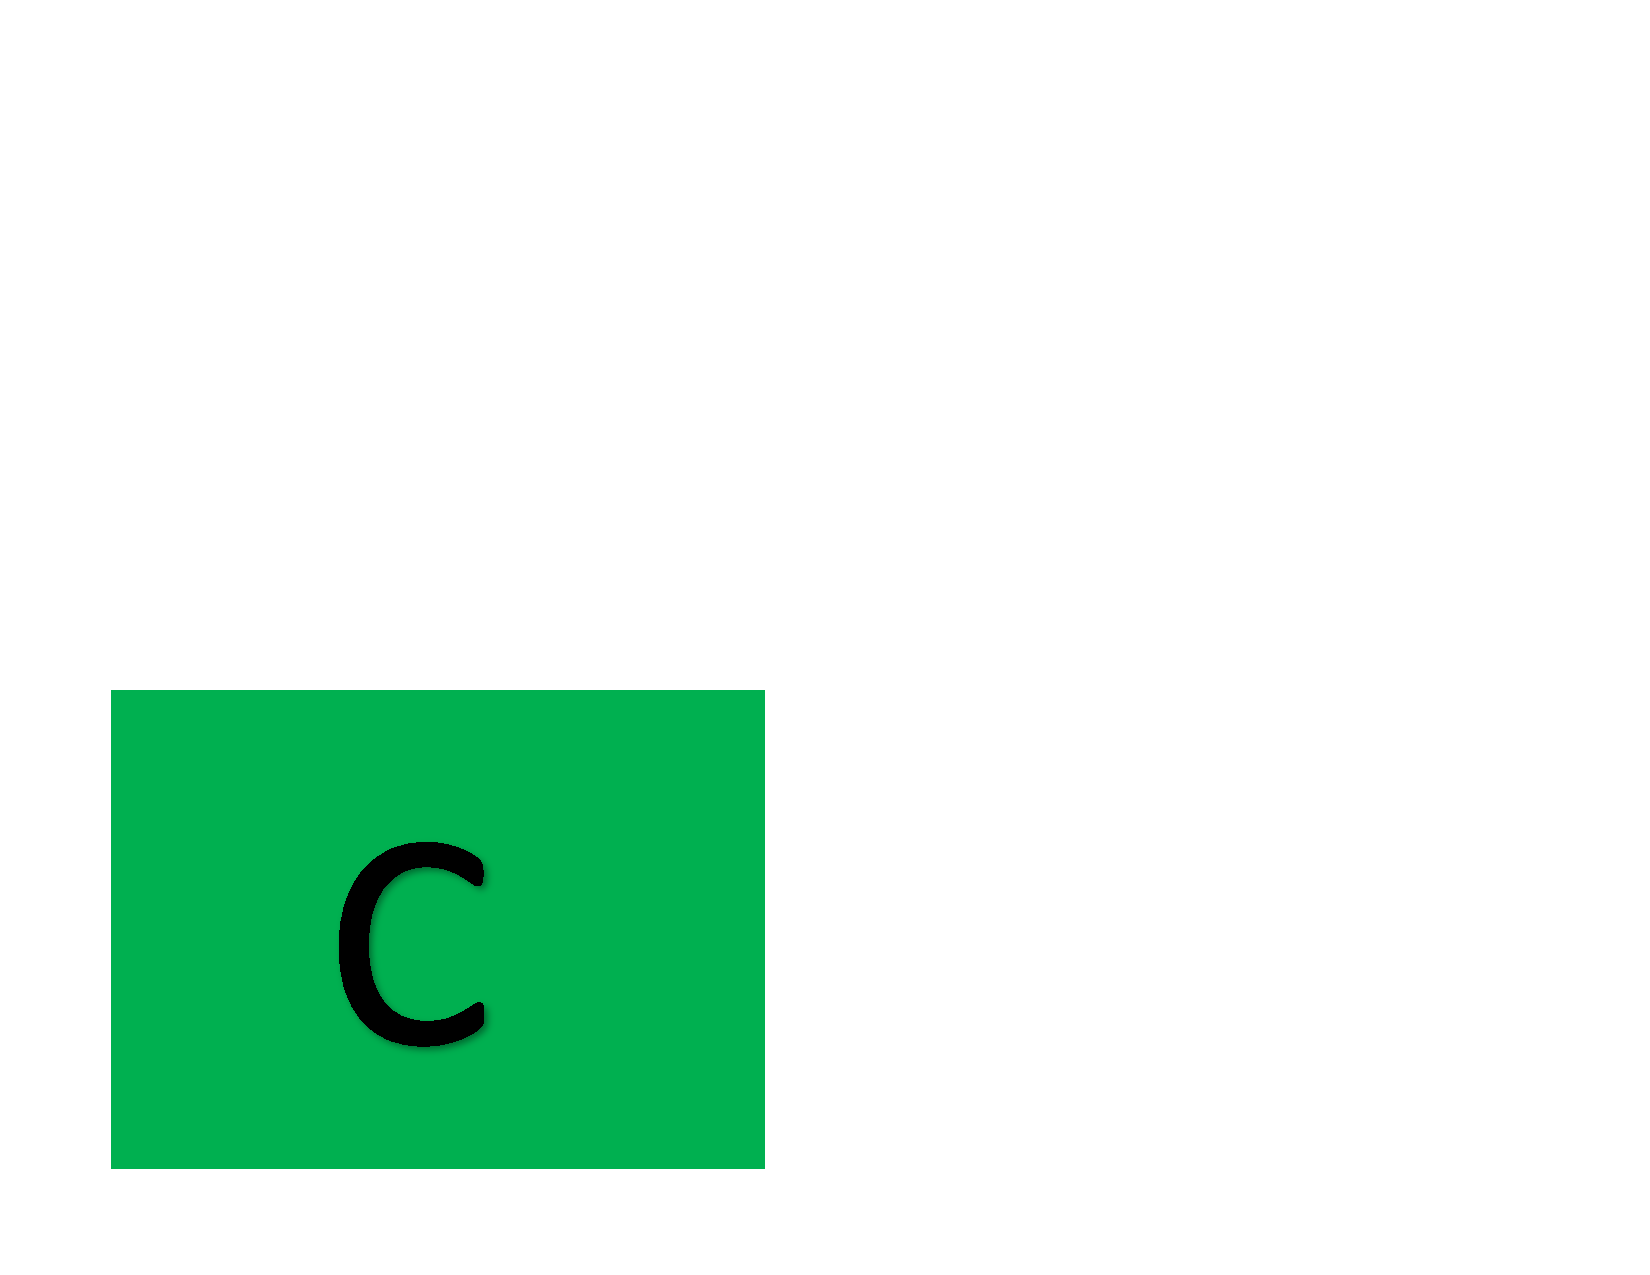
\includegraphics[width=0.8cm,height=0.5cm]{figures/C}} ]  }
\newcommand*{\ditem}{ \item[{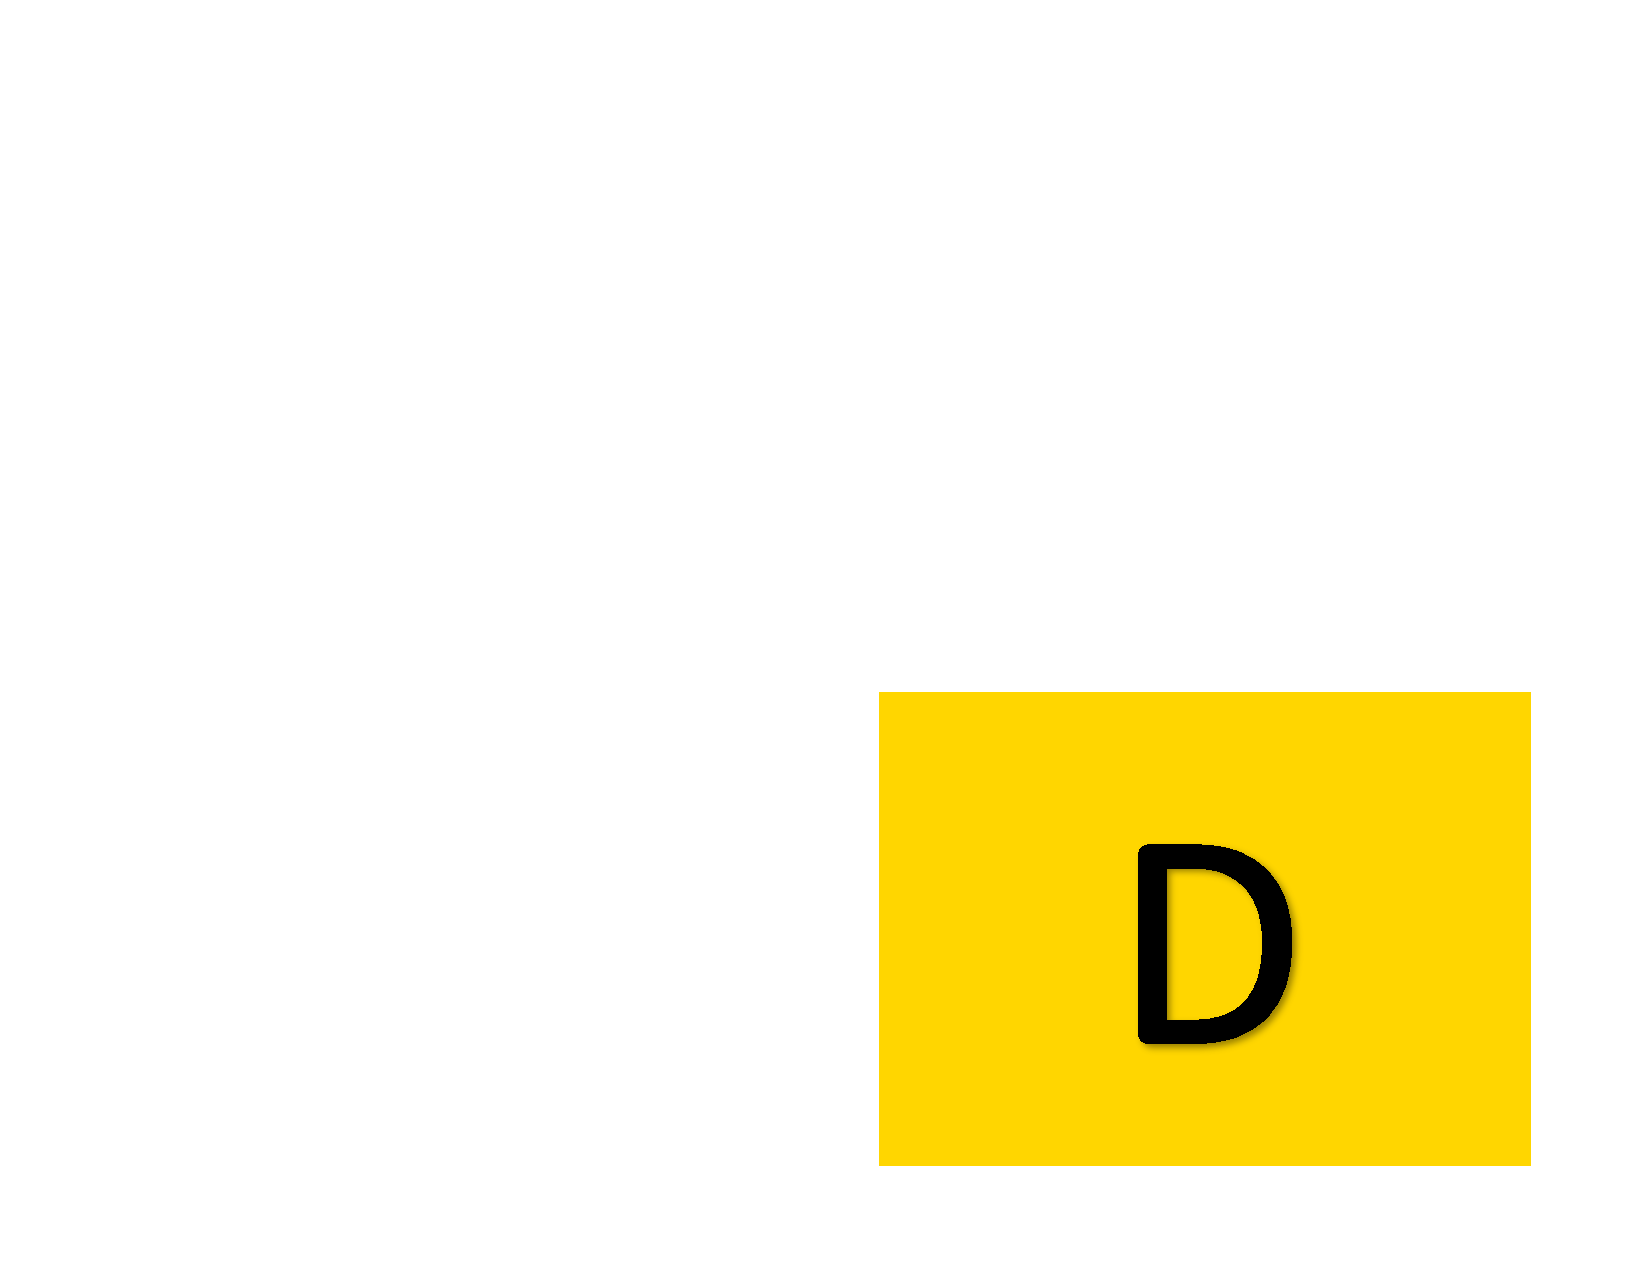
\includegraphics[width=0.8cm,height=0.5cm]{figures/D}} ]  }
\newcommand*{\eitem}{ \item[{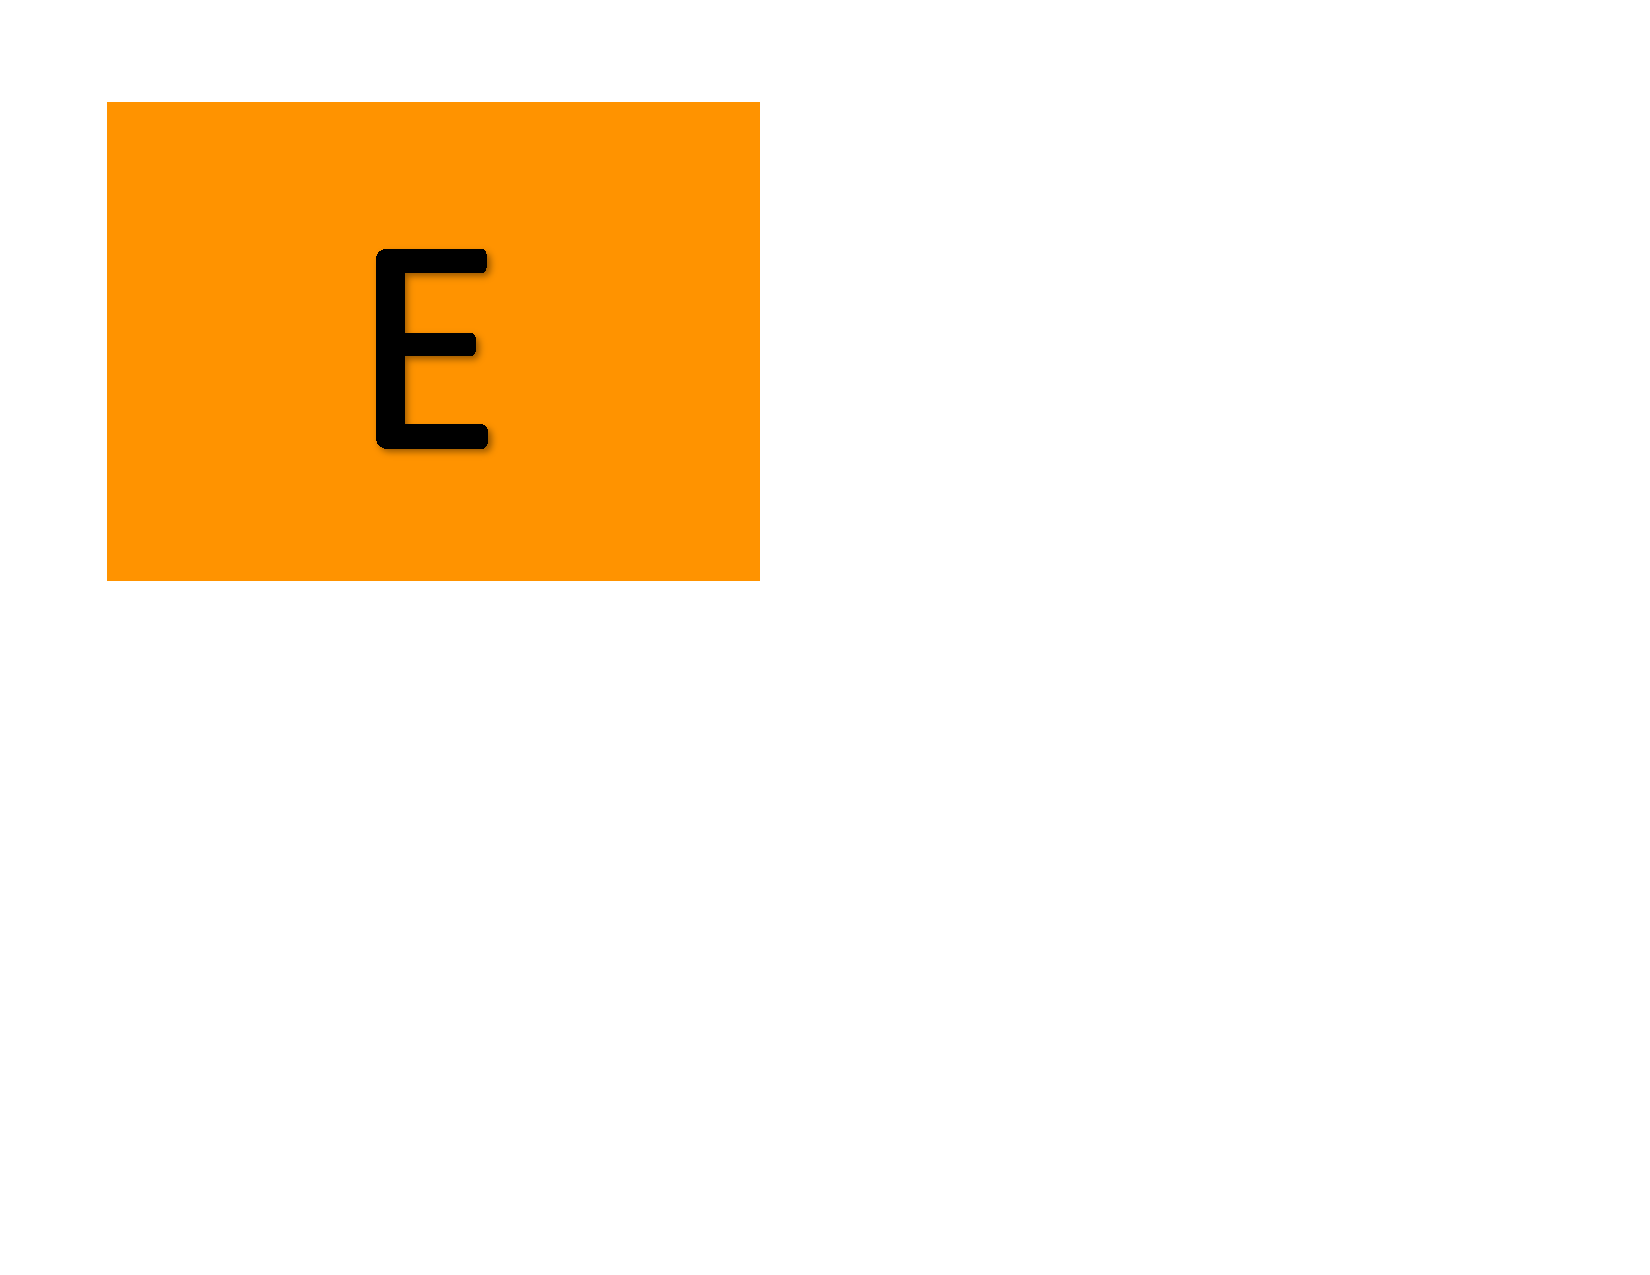
\includegraphics[width=0.8cm,height=0.5cm]{figures/E}} ]  }
\newcommand*{\fitem}{ \item[{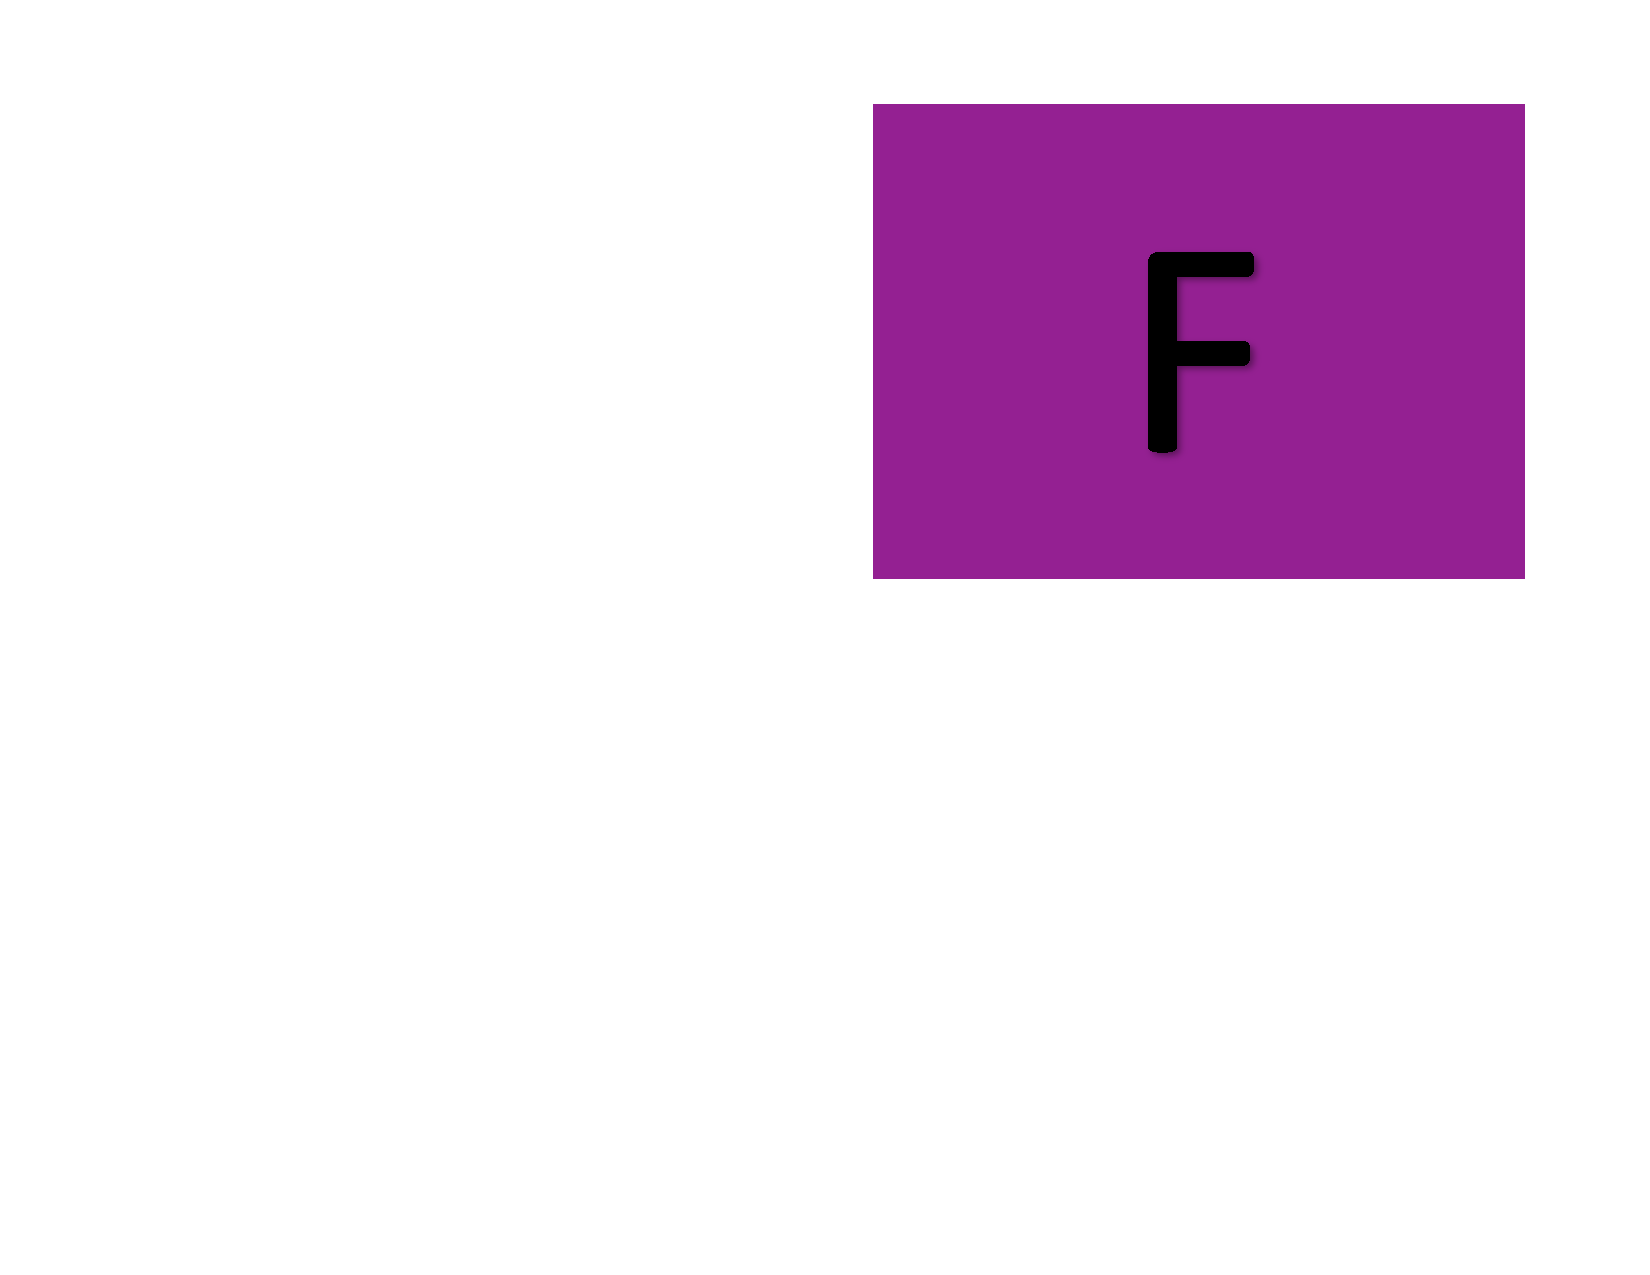
\includegraphics[width=0.8cm,height=0.5cm]{figures/F}} ]  }


\newcommand{\hide}[1]{\underline{\phantom{#1 #1}}}

\usepackage{setspace}

\onehalfspacing

\begin{document}
    \sweek{11b: Beyond NP, Undecidability, and Time Hierarchy}{November 5, 2026}

    \section{Decision problems and undecidability}
    A decision problem $Q$ is \emph{undecidable} if there cannot exist an algorithm that always halts and provides the correct YES or NO answer.

    \begin{Qu}
        Say that $Q$ is an NP-Complete problem. Which of the following statements is true?
        \begin{itemize}
            \aitem $Q$ is undecidable
            \bitem If $P \neq NP$, then $Q$ is undecidable, but we just do not know for sure yet
            \citem Neither of the above is true
        \end{itemize}
    \end{Qu}
    % Answer: (c). Enumerating all polynomial-length certificates gives
    % a decider, even if finding an accepting certificate takes a long time.


%\vfill
%Question: Are NP-hard problems the hardest problems that exist? Can anything be harder?
\newpage

\section{Halting and the Halting Problem}
Let $P$ represent some notion of a computer program and $I$ represent some type of input that you give $P$. You can think of both as strings.\\

We say that $P$ \emph{halts} on $I$ if \hide{running $P$ on input $I$ eventually terminates.} \\

\paragraph{Example}
Let $P = \textsc{OddHello}$ be represented by the following code snippet.
\begin{algorithm}[h]
    \textsc{OddHello}($I$)
    \begin{algorithmic}
        \If{the input is a string with an even number of letter characters (a-z)}
        \While{true}
        \State continue
        \EndWhile
        \Else
        \State return ``hello!''
        \EndIf
    \end{algorithmic}
\end{algorithm}
% iftheinputisastringwithanevennumberoflettercharactersazthenwhiletruedocontinueendwhileelseReturnHelloendif has 101 characters

\begin{Qu}
    Does $\langle P, I\rangle$ halt when $I$ = ``hello''?
    \begin{itemize}
        \aitem Yes
        \bitem Nope
        \citem It depends
        \ditem There is no way of knowing
    \end{itemize}
\end{Qu}
% Answer: (a).

\begin{Qu}
Does $\langle P, I\rangle$ halt when $I$ = ``hi''?
    \begin{itemize}
        \aitem Yes
        \bitem Nope
        \citem It depends
        \ditem There is no way of knowing
    \end{itemize}
\end{Qu}
% Answer: (b).

For the next question, suppose our fixed text representation of $P$ contains $101$ lowercase letters.
\begin{Qu}
    Does $\langle P, I\rangle$ halt when $I$ = $P$?
    \begin{itemize}
        \aitem Yes
        \bitem Nope
        \citem This question cannot have an answer
    \end{itemize}
\end{Qu}
% Answer: (a). A program description is a string and can be used as input.

\vspace{1cm}

\newpage

\textbf{Definition: The Halting Problem.} The \emph{halting problem} is a decision problem that takes in inputs of the form $\langle P, I \rangle$ and outputs
\begin{itemize}
    \item YES \\ \\%if P halts on I
    \item NO \\%if P does not halt on I
\end{itemize}

\emph{To be clear}
\begin{itemize}
    \item An instance of the halting problem is given by a \\ \\
    % program P and an input I.
    \item An algorithm $A$ solves the halting problem if
    % for every program-input pair (P,I), it halts and correctly answers
    % whether or not P halts on I.
\end{itemize}

\newpage

\begin{theorem} The Halting Problem is \hide{undecidable.}
\end{theorem}

\textit{Proof.} Suppose there is an algorithm $H$ that always halts and correctly solves the halting problem. Thus,
\begin{itemize}
    \item $H(M,I)$ returns YES if \hide{$M$ halts on $I$.}
    \item $H(M,I)$ returns NO if \hide{$M$ does not halt on $I$.}
\end{itemize}

We can represent the code of a program $M$ as a string $\langle M\rangle$. This string can also be used as the input to a program.

\paragraph{A new program}
Using $H$, construct the following program.
\begin{algorithm}[h]
    \textsc{Opposite}($z$)
    \begin{algorithmic}
        \If{$z$ is not a valid program description}
            \State return
        \EndIf
        \If{$H(z,z)$ returns YES}
            \While{true}
                \State continue
            \EndWhile
        \Else
            \State return
        \EndIf
    \end{algorithmic}
\end{algorithm}

\textbf{Observation.} Here $H(z,z)$ asks whether the program described by $z$ halts when its input is the string $z$.

\newpage
\subsection*{Running a program on its own description}
Let $b=\langle\textsc{Opposite}\rangle$ be the description of our new program. What happens when we run \textsc{Opposite}$(b)$?

\begin{itemize}
    \item Suppose $H(b,b)$ returns YES. What does $H$ predict, and what does \textsc{Opposite} actually do?
    \vs{2cm}
    % H predicts that Opposite(b) halts, but Opposite(b) loops forever.
    \item Suppose $H(b,b)$ returns NO. What does $H$ predict, and what does \textsc{Opposite} actually do?
    \vs{2cm}
    % H predicts that Opposite(b) does not halt, but Opposite(b) returns.
\end{itemize}

In either case, \hide{$H$ gives an incorrect answer.} Therefore, no such algorithm $H$ exists.

\paragraph{What if we impose a deadline?}
\begin{Qu}
    Given a program $M$, an input $I$, and a positive integer $T$, can an algorithm always decide whether $M$ halts on $I$ within $T$ steps?
    \begin{itemize}
        \aitem Yes
        \bitem No, because the halting problem is undecidable
        \citem Only if $M$ eventually halts on $I$
    \end{itemize}
\end{Qu}
% Answer: (a). Simulate M for T steps, stopping early if it halts.

\vfill
We will return to deadlines later. First, we will study decidable problems using another measure of computational resources: memory.


\newpage
\section{Space Complexity}
So far, we have measured how many steps an algorithm takes. We can also measure how much memory it uses.

\paragraph{Example}
Suppose we solve SAT by trying all assignments to $n$ Boolean variables.
\begin{itemize}
    \item How many assignments are there? \hide{$2^n$.}
    \item How many bits are needed to store one assignment? \hide{$n$.}
    \item Do we need to keep all the assignments in memory at once?
\end{itemize}
\vs{1cm}

The \emph{space complexity} of an algorithm measures the largest amount of workspace it uses at any one time. We include counters and the recursion stack, but do not count the read-only input.

\textbf{Definition.} The class $\mathrm{PSPACE}$ consists of decision problems solvable by a deterministic algorithm that always halts and uses polynomial space.

\begin{theorem}
    $\mathrm{P}\subseteq\mathrm{PSPACE}$.
\end{theorem}
\textit{Proof.} How much workspace can an algorithm visit in a polynomial number of steps?
\vs{1.5cm}
% A machine with a fixed number of tapes visits at most O(t(n)+1)
% work cells in t(n) steps.

\newpage
\subsection*{What about NP?}
\begin{theorem}
    $\mathrm{NP}\subseteq\mathrm{PSPACE}$.
\end{theorem}

\textit{Proof.} Let $Q\in\mathrm{NP}$. There is a polynomial-time verifier $V$ and a polynomial $p$ such that
\begin{equation*}
    x\in Q \iff V(x,y)\text{ accepts for some }y\text{ with }|y|\leq p(|x|).
\end{equation*}

\paragraph{The algorithm}
\begin{itemize}
    \item Enumerate all binary strings $y$ of length at most $p(|x|)$, one at a time.
    \item For each $y$, run $V(x,y)$. Accept if it accepts.
    \item If no candidate is accepted, reject.
\end{itemize}

\paragraph{Account for the space}
What do we need to keep in memory? Which workspace can we reuse?
\vs{2cm}
% The current candidate and enumeration counters use polynomial space.
% The verifier uses polynomial time, hence polynomial space, because
% |y| is polynomial in |x|. Reuse its workspace for each candidate.

\begin{Qu}
    Why does the exponential number of possible certificates not force exponential space?
    \begin{itemize}
        \aitem We only need to store one candidate and one verifier computation at a time
        \bitem Every NP problem has only polynomially many certificates
        \citem Exponential time always implies polynomial space
    \end{itemize}
\end{Qu}
% Answer: (a).


\newpage
\section{Quantified Boolean Formulas}
Recall that SAT asks whether there is an assignment that makes a Boolean formula true. We can write this as
\begin{equation*}
    \exists x_1\exists x_2\cdots\exists x_m\ \varphi(x_1,\ldots,x_m).
\end{equation*}

What changes if some variables must work for \emph{both} possible values?
\begin{itemize}
    \item $\exists x\,\varphi(x)$ is true if \hide{at least one choice of $x$ makes $\varphi$ true.}
    \vs{.5cm}
    \item $\forall x\,\varphi(x)$ is true if \hide{both choices of $x$ make $\varphi$ true.}
\end{itemize}

\paragraph{Example}
Consider
\begin{equation*}
    \forall x\exists y\ (x\leftrightarrow y).
\end{equation*}
Here $x\leftrightarrow y$ is true exactly when $x$ and $y$ have the same value.

\begin{Qu}
    Is this quantified formula true?
    \begin{itemize}
        \aitem Yes
        \bitem No
    \end{itemize}
\end{Qu}
What choice of $y$ works for each value of $x$?
\vs{1cm}
% Answer: (a). Set y=x.

\newpage
\subsection*{The order of the quantifiers matters}
Now reverse the order:
\begin{equation*}
    \exists y\forall x\ (x\leftrightarrow y).
\end{equation*}

\begin{Qu}
    Is this quantified formula true?
    \begin{itemize}
        \aitem Yes
        \bitem No
    \end{itemize}
\end{Qu}
Explain why changing the order changes the answer.
\vs{1.5cm}
% Answer: (b). After y is fixed, choose x=1-y.

\paragraph{A game interpretation}
There are two players, True and False. Read the quantifiers from left to right.
\begin{itemize}
    \item True chooses the value of each variable with an $\exists$ quantifier.
    \item False chooses the value of each variable with a $\forall$ quantifier.
    \item Each player sees all earlier choices.
    \item True wins if the resulting Boolean formula evaluates to true.
\end{itemize}

The quantified formula is true exactly when \hide{True has a winning strategy.}

\vfill
\textbf{Observation.} An existential choice can depend on earlier universal choices, but cannot depend on choices that have not been made yet.

\newpage
\section{True Quantified Boolean Formula}
An input to \textsc{TQBF} has the form
\begin{equation*}
    Q_1x_1Q_2x_2\cdots Q_mx_m\ \varphi(x_1,\ldots,x_m),
\end{equation*}
where every $Q_i$ is either $\exists$ or $\forall$, and every variable is quantified. The decision problem asks whether the quantified formula is true.

\begin{center}
    \textsc{TQBF} $=\phantom{\{\langle\Phi\rangle:\Phi\text{ is a true quantified Boolean formula}\}}$
\end{center}

\paragraph{Example}
Consider the formula
\begin{equation*}
    \exists x\forall y\exists z\ \big[(x\lor y)\land(y\leftrightarrow z)\big].
\end{equation*}
Does True have a winning strategy? Specify the first choice and how the last choice depends on False's move.
\vs{2cm}
% True chooses x=1, then z=y.

\paragraph{Evaluating the game tree}
Try both values of the next variable and recursively evaluate what remains.
\begin{itemize}
    \item At an $\exists$ node, combine the two answers using \hide{OR.}
    \item At a $\forall$ node, combine the two answers using \hide{AND.}
\end{itemize}

\newpage
\subsection*{How much space does the game tree need?}
\begin{theorem}
    $\textsc{TQBF}\in\mathrm{PSPACE}$.
\end{theorem}

\textit{Proof.} Evaluate the tree using depth-first search. At each node, evaluate the first child, remember its answer, and then evaluate the second child.

\paragraph{Account for the space}
Let $n$ be the length of the input formula and $m\leq n$ its number of variables.
\begin{itemize}
    \item How deep is the recursion? \hide{$m$ levels.}
    \vs{.5cm}
    \item What must we remember about the assignments on the current path?
    \vs{1cm}
    \item After evaluating the first child, how much of its subtree must we keep while evaluating the second child?
    \vs{1cm}
\end{itemize}
% Keep the current partial assignment, the next child to explore, and
% one returned answer per level. Indices use O(log n) bits per frame.
% Reuse the workspace for each child. Evaluate the matrix in polynomial
% space at each leaf. The original formula stays on the read-only input.

There can be $2^m$ leaves, but we do not store the whole tree. The current path, recursion stack, and workspace for evaluating $\varphi$ all take polynomial space in $n$.

\vfill
\textbf{Observation.} As with enumerating SAT assignments, a large number of possibilities does not mean that all possibilities must be stored at once.


\newpage
\subsection*{PSPACE-completeness}
A decision problem $Q$ is \emph{PSPACE-complete} if:
\begin{itemize}
    \item $Q\in\mathrm{PSPACE}$; and
    \item Every problem in $\mathrm{PSPACE}$ has a polynomial-time reduction to $Q$.
\end{itemize}

\begin{theorem}
    \textsc{TQBF} is \hide{PSPACE-complete.}
\end{theorem}
We proved that $\textsc{TQBF}\in\mathrm{PSPACE}$. We will use the hardness part as a known theorem, without giving the reductions.

\begin{Qu}
    Suppose someone finds a polynomial-time algorithm for \textsc{TQBF}. What follows?
    \begin{itemize}
        \aitem Only \textsc{TQBF} becomes easy
        \bitem Every problem in $\mathrm{PSPACE}$ can be solved in polynomial time
        \citem Every decidable problem can be solved in polynomial time
        \ditem The halting problem becomes decidable
    \end{itemize}
\end{Qu}
% Answer: (b). Compose a polynomial-time reduction with the assumed solver.

\paragraph{Use the containments we have proved}
Under this hypothesis, fill in the relationships:
\begin{equation*}
    \mathrm{P}\ \hide{=}\ \mathrm{NP}\ \hide{=}\ \mathrm{PSPACE}.
\end{equation*}
Explain where we used PSPACE-completeness.
\vs{1.5cm}
% Every problem in PSPACE reduces to TQBF in polynomial time.
% The reduction's output has polynomial length, so the composition
% with the assumed polynomial-time TQBF algorithm is polynomial-time.

\vfill
We have seen that a problem can be solved using a modest amount of memory while taking a very large number of steps. Next, we will place an upper bound on that running time.

\newpage
\section{Exponential Time}
The class $\mathrm{EXPTIME}$ consists of decision problems that can be solved by a deterministic algorithm in time $2^{p(n)}$ for some polynomial $p$, where $n$ is the input length.

\paragraph{Examples of allowed time bounds}
\begin{equation*}
    2^n, \qquad 2^{n^2}, \qquad 2^{n^3}.
\end{equation*}

\begin{theorem}
    $\mathrm{P}\subseteq\mathrm{EXPTIME}$.
\end{theorem}
\textit{Proof.}
\vs{1.5cm}
% Every polynomial running time is bounded by 2^{p(n)} for a suitable polynomial p.

\begin{Qu}
    An algorithm takes $2^n$ steps to solve a decision problem $Q$. Does this prove that $Q\notin\mathrm{P}$?
    \begin{itemize}
        \aitem Yes, because $2^n$ is not polynomial
        \bitem No, because there might be a faster algorithm for $Q$
        \citem No, because $2^n$ is polynomial
    \end{itemize}
\end{Qu}
% Answer: (b).

\paragraph{Example}
A program waits for $2^n$ steps, then accepts if its input begins with $1$ and rejects otherwise. It rejects the empty string. How quickly could we solve the same problem?
\vs{1cm}
% Check the first symbol immediately.


\newpage
\section{Relating Space and Time}
A polynomial-space algorithm might take much longer than polynomial time. How long could it run before it must repeat itself?

\paragraph{A small example}
Suppose a deterministic machine has:
\begin{itemize}
    \item $3$ possible internal states;
    \item $4$ work-tape cells, each containing one bit;
    \item a work-tape head pointing to one of the $4$ cells.
\end{itemize}
For this example, its input head stays fixed.

How many different complete snapshots of this machine are possible?
\begin{equation*}
    \hide{3\cdot 4\cdot 2^4=192.}
\end{equation*}

\paragraph{Configurations}
A \emph{configuration} records everything needed to determine the next step: the internal state, the tape contents, and all head positions. We consider a fixed input.

\begin{Qu}
    If a deterministic machine repeats a configuration before halting, what happens?
    \begin{itemize}
        \aitem It must halt at the next step
        \bitem It repeats the same computation and loops forever
        \citem It may choose a different next step the second time
    \end{itemize}
\end{Qu}
% Answer: (b).

\newpage
\subsection*{Polynomial space gives an exponential time bound}
\begin{theorem}
    $\mathrm{PSPACE}\subseteq\mathrm{EXPTIME}$.
\end{theorem}

\textit{Proof.} Fix a deterministic decider and an input of length $n$. Suppose the machine uses at most $s(n)\geq 1$ work-tape cells, where $s$ is polynomial.

For simplicity, use one work tape. The input head stays between the two input endmarkers. Let $q$ be the number of internal states and $\Gamma$ the work-tape alphabet. Both are constants for this machine.

\paragraph{Count the configurations}
\begin{itemize}
    \item Internal state: \hide{$q$ possibilities.}
    \item Input-head position: \hide{$n+2$ possibilities.}
    \item Work-head position: \hide{$s(n)$ possibilities.}
    \item Work-tape contents: \hide{$|\Gamma|^{s(n)}$ possibilities.}
\end{itemize}

Therefore, the number of configurations is at most
\begin{equation*}
    q(n+2)s(n)|\Gamma|^{s(n)}\leq\hide{2^{p(n)}}
\end{equation*}
for some polynomial $p$.

Why can the decider not repeat a configuration before halting?
\vs{1.5cm}
% Repetition would force an infinite loop, but a decider always halts.

Thus, its running time is bounded by the number of possible configurations, which is exponential in a polynomial in $n$.
% A fixed number of work tapes changes the count but not this conclusion.


\begin{equation*}
    \mathrm{P}\subseteq\mathrm{NP}\subseteq\mathrm{PSPACE}\subseteq\mathrm{EXPTIME}.
\end{equation*}
Which of these containments are strict? We will return to this question after studying an EXPTIME-complete problem.

\newpage
\section{Games and Exponential Time}
In \textsc{TQBF}, two players choose Boolean values, and each play has only one move per variable. What happens when a game can continue for many more moves?

\paragraph{A reachability game}
Two players, Alice and Bob, move a token between positions. Each position specifies whose turn it is and two possible next positions.
\begin{itemize}
    \item Alice wins if the token reaches a goal position.
    \item Bob wins if the token never reaches a goal position.
\end{itemize}
Both players know the current position and all earlier moves. A strategy tells a player which move to make after each possible history.

\paragraph{Play with a neighbor}
The token begins at $s$. The goal is $g$. A position $\ell$ is a losing trap: both moves from $\ell$ return to $\ell$.
\begin{center}
    \begin{tabular}{c|c|c|c}
        Position & Whose turn? & First move & Second move \\
        \hline
        $s$ & Alice & $a$ & $b$ \\
        $a$ & Bob & $g$ & $\ell$ \\
        $b$ & Alice & $g$ & $\ell$ \\
        $\ell$ & Bob & $\ell$ & $\ell$
    \end{tabular}
\end{center}
Which first move lets Alice force a win? What happens if Alice chooses the other first move?
\vs{1.5cm}
% Alice chooses b, then g. If she chooses a, Bob chooses the trap ell.

\vfill
\textbf{Observation.} Having some sequence of moves that reaches the goal is different from having a strategy that wins against every response by the opponent.

\newpage
\subsection*{Describing a large game}
For the problem below, a position is a string of $k$ bits. Thus there are \hide{$2^k$ possible positions.} We describe the rules compactly, instead of listing all positions and moves.

\paragraph{The input}
An instance consists of an initial position $s_0\in\{0,1\}^k$ and Boolean circuits specifying:
\begin{itemize}
    \item $O(s)$: whose turn it is at position $s$ ($0$ for Alice, $1$ for Bob);
    \item $G(s)$: whether $s$ is a goal position;
    \item $N_0(s)$ and $N_1(s)$: the two possible next positions, each a $k$-bit string.
\end{itemize}
A Boolean circuit is a finite acyclic network of AND, OR, and NOT gates. We can evaluate it in time polynomial in its description length.

\paragraph{The rules}
At a goal position, Alice immediately wins. Otherwise, the player whose turn it is chooses one of the two next positions. If play continues forever without reaching a goal, Bob wins. The two next positions are allowed to be the same.

\textbf{Definition.} The decision problem \textsc{Games} asks whether Alice has a winning strategy from $s_0$.
\begin{center}
    \textsc{Games} $=\phantom{\{\langle s_0,O,G,N_0,N_1\rangle:\text{Alice has a winning strategy}\}}$
\end{center}

\textbf{To be clear.} The input is the initial position and the circuits. Its length is not the number of positions in the game.

\begin{theorem}
    \textsc{Games} is \hide{EXPTIME-complete.}
\end{theorem}
This means that \textsc{Games} belongs to $\mathrm{EXPTIME}$ and every problem in $\mathrm{EXPTIME}$ has a polynomial-time reduction to \textsc{Games}. We will use hardness as a known theorem and prove membership next.
% This is succinct two-player reachability, not an explicitly listed game graph.
% EXPTIME-hardness follows from APSPACE=EXPTIME (Chandra--Kozen--Stockmeyer):
% encode polynomial-space alternating-machine configurations as positions,
% existential/universal states as Alice/Bob, and accepting states as goals.
% The owner, goal, and two transition functions have polynomial-size circuits.
% Rejecting configurations are non-goal traps; malformed configurations can
% also be made traps. Source: https://research.ibm.com/publications/alternation

\newpage
\subsection*{Finding the winning positions}
\begin{theorem}
    $\textsc{Games}\in\mathrm{EXPTIME}$.
\end{theorem}

\textit{Proof.} Enumerate the $2^k$ positions. Initially, mark all goal positions as winning for Alice. Repeatedly apply the following rules:
\begin{itemize}
    \item If it is Alice's turn, mark the position when: 
		%\hide{at least one successor is marked.}
    \vs{.5cm}
    \item If it is Bob's turn, mark the position when:
		%\hide{both successors are marked.}
		\vs{.5cm}
\end{itemize}
In each round, use the marks from the previous round. Stop when a round adds no new marks. Answer YES exactly when $s_0$ is marked.

\paragraph{Why are the marked positions winning?}
Think about the round in which a position was first marked. Can Alice ensure that this round number decreases after each move, until the goal is reached?
\vs{1cm}
% At an Alice position she selects a successor marked in an earlier round.
% At a Bob position both successors were marked in an earlier round.

\paragraph{What about an unmarked position?}
After the process stops, can Bob keep the token outside the marked set?
\vs{1cm}
% Every unmarked Alice position has both successors unmarked.
% Every unmarked Bob position has at least one unmarked successor.
% Bob can therefore prevent reaching any goal forever.

\paragraph{Running time}
There are at most \hide{$2^k$ rounds that add new positions.} Each round takes polynomial time in the size of the explicit position table and the circuit descriptions. If $n$ is the total input length, then $k\leq n$, and the total running time is
\begin{equation*}
    (2^k+n)^{O(1)}=2^{\mathrm{poly}(n)}.
\end{equation*}
% Even a polynomial overhead for accessing the explicit marked-state table
% on a Turing machine preserves an exponential-time bound.

\vfill
\textbf{Observation.} If the whole game graph were explicitly listed, this procedure would take polynomial time in the size of that graph. The compact representation is essential here.

\newpage
\section{Separating P and EXPTIME}
\begin{theorem}
    $\mathrm{P}\subsetneq\mathrm{EXPTIME}$.
\end{theorem}

To prove this theorem, we need a decision problem $D$ such that:
\begin{itemize}
    \item There is \hide{an exponential-time algorithm for $D$.}
    \item There is no \hide{polynomial-time algorithm for $D$.}
\end{itemize}

We will use the same idea as in the halting problem proof: run a program on its own description and give the opposite answer. This time, we will stop the simulation after a fixed number of steps.

\paragraph{The input}
An input has the form
\begin{equation*}
    w=\langle M\rangle\#1^r,
\end{equation*}
where $\langle M\rangle$ describes a deterministic program, $\#$ separates its code from the padding, and $1^r$ is a string of $r$ ones.

The input length is $n=|w|$, including the padding.

\paragraph{Why include extra ones?}
The code for $M$ stays the same, but we can make the input as long as we like by increasing $r$.

\vs{1cm}
\textbf{To be clear.} We will run $M$ on the entire string $w$, including its own description and the padding. The program $M$ need not recognize the input as its own code.

\newpage
\subsection*{A problem that gives the opposite answer}
Define $D$ to be the set of strings accepted by the following algorithm.

\begin{algorithm}[h]
    \textsc{Diagonal}($w$)
    \begin{algorithmic}
        \If{$w$ is not of the form $\langle M\rangle\#1^r$}
            \State reject
        \EndIf
        \State Let $n=|w|$
        \State Simulate $M$ on input $w$ for at most $2^n$ steps of $M$
        \If{$M$ accepts within those $2^n$ steps}
            \State reject
        \Else
            \State accept
        \EndIf
    \end{algorithmic}
\end{algorithm}

\begin{Qu}
    What does \textsc{Diagonal} output in each case?
    \begin{itemize}
        \aitem $M(w)$ accepts by the deadline: \hide{NO}
        \bitem $M(w)$ rejects by the deadline: \hide{YES}
        \citem $M(w)$ is still running at the deadline: \hide{YES}
    \end{itemize}
\end{Qu}

\paragraph{First, show that $D\in\mathrm{EXPTIME}$}
Why does \textsc{Diagonal} always halt?
\vs{1cm}
% The simulation stops at the deadline even if M never halts.

We use the fact that a simulator can carry out $T$ steps of a program in time polynomial in $n+T$, when the program description and its input each have length at most $n$. Thus, the total running time is
\begin{equation*}
    (n+2^n)^{O(1)}=\hide{2^{O(n)}}.
\end{equation*}
% This bound includes the clock. Simulated steps and simulator steps differ.

\newpage
\subsection*{Could a polynomial-time algorithm solve D?}
Suppose an algorithm $A$ correctly decides $D$ in time $q(n)$ for some polynomial $q$.

Choose the input
\begin{equation*}
    w=\langle A\rangle\#1^r, \qquad n=|w|.
\end{equation*}

\paragraph{Choosing the padding}
How large should $r$ be? We want
\begin{equation*}
    \hide{q(n)<2^n.}
\end{equation*}
Why is it possible to arrange this?
\vs{1cm}
% A and q are fixed, while the padding lets n grow arbitrarily large.
% Eventually 2^n exceeds q(n).

With this choice, $A(w)$ finishes before the deadline. There are two cases:
\begin{itemize}
    \item If $A(w)$ accepts, the definition of $D$ says that $w$ \hide{is not in $D$.}
    \vs{.5cm}
    \item If $A(w)$ rejects, the definition of $D$ says that $w$ \hide{is in $D$.}
\end{itemize}

Therefore, \hide{$A$ gives the wrong answer on $w$.} This contradicts the assumption that $A$ decides $D$.

\vfill
We have shown that $D\in\mathrm{EXPTIME}$ and $D\notin\mathrm{P}$. Hence,
\begin{equation*}
    \mathrm{P}\subsetneq\mathrm{EXPTIME}.
\end{equation*}

\newpage
\subsection*{What made the argument work?}
\begin{Qu}
    Why did we add padding instead of using only $\langle A\rangle$?
    \begin{itemize}
        \aitem A program cannot take its own code as input without padding
        \bitem The unpadded input might be too short for $q(n)<2^n$ to hold
        \citem Adding padding changes $A$ into a faster program
        \ditem Padding makes an undecidable problem decidable
    \end{itemize}
\end{Qu}
% Answer: (b).

\vs{.5cm}
\begin{Qu}
    Does \textsc{Diagonal} need to know the polynomial $q(n)$?
    \begin{itemize}
        \aitem Yes, to choose its deadline
        \bitem No, its deadline is always $2^n$
        \citem Yes, to decide whether $w$ is a valid input
    \end{itemize}
\end{Qu}
% Answer: (b). The proof uses q only to choose a failing input for A.

\paragraph{Compare with the halting problem}
\begin{itemize}
    \item For the halting problem, we ruled out \hide{every algorithm that always halts and is correct.}
    \vs{.5cm}
    \item For $D$, we ruled out \hide{every polynomial-time algorithm that is correct.}
\end{itemize}

\vfill
This method of making a program disagree with a proposed solver on a description of that solver is called \hide{diagonalization.}


\newpage
\subsection*{What does the separation tell us?}
We have proved that
\begin{equation*}
    \mathrm{P}\subseteq\mathrm{NP}\subseteq\mathrm{PSPACE}\subseteq\mathrm{EXPTIME},
\end{equation*}
and that $\mathrm{P}\neq\mathrm{EXPTIME}$.

\begin{Qu}
    Which conclusion must follow?
    \begin{itemize}
        \aitem $\mathrm{P}\neq\mathrm{NP}$
        \bitem $\mathrm{NP}\neq\mathrm{PSPACE}$
        \citem $\mathrm{PSPACE}\neq\mathrm{EXPTIME}$
        \ditem At least one of the three containments is strict
    \end{itemize}
\end{Qu}
% Answer: (d).

\paragraph{Return to Games}
Could \textsc{Games} have a polynomial-time algorithm?
\vs{1.5cm}
% No. By EXPTIME-completeness, every EXPTIME problem would then have
% a polynomial-time algorithm, contradicting P != EXPTIME.

\paragraph{Return to TQBF}
If \textsc{TQBF} had a polynomial-time algorithm, what would the chain become? Fill each blank with $=$ or $\subsetneq$.
\begin{equation*}
    \mathrm{P}\ \hide{=}\ \mathrm{NP}\ \hide{=}\ \mathrm{PSPACE}\ \hide{\subsetneq}\ \mathrm{EXPTIME}.
\end{equation*}
\vs{1cm}
% PSPACE-completeness collapses the first three classes. The last inclusion
% is still strict because the first class differs from EXPTIME.

\newpage
\section{The Time Hierarchy Theorem}
We have shown that exponential time lets us solve some problems that polynomial time does not. Can the same idea separate other running-time bounds?

Write $\mathrm{DTIME}(t(n))$ for the decision problems solvable by a deterministic algorithm in $O(t(n))$ time. For this theorem, we use the standard multitape Turing-machine model.

\paragraph{Constructing a clock}
A function $t(n)\geq n$ is \emph{time-constructible} if, on input $1^n$, a machine can write $1^{t(n)}$ in $O(t(n))$ time. We can use these $t(n)$ marks to count steps. The bounds $n^2$, $n^3$, and $2^n$ are examples.

\begin{theorem}[Deterministic Time Hierarchy Theorem]
    Let $t(n),T(n)\geq n$ be time-constructible functions. If
    \begin{equation*}
        t(n)\log t(n)=o(T(n)),
    \end{equation*}
    then
    \begin{equation*}
        \mathrm{DTIME}(t(n))\subsetneq\mathrm{DTIME}(T(n)).
    \end{equation*}
\end{theorem}
Here $f(n)=o(g(n))$ means that $f(n)/g(n)$ tends to zero as $n$ grows.

\paragraph{Example}
Since $n^2\log(n^2)=o(n^3)$, the theorem gives
\begin{equation*}
    \mathrm{DTIME}(n^2)\ \hide{\subsetneq}\ \mathrm{DTIME}(n^3).
\end{equation*}
Does a problem separating these two classes have to be outside $\mathrm{P}$?
\vs{1cm}
% No. The O(n^3)-time algorithm is still polynomial-time.

\newpage
\subsection*{Accounting for the simulation}
\textit{Proof of the time hierarchy theorem.} We will construct a decision problem $D_T$ that belongs to $\mathrm{DTIME}(T(n))$ but not to $\mathrm{DTIME}(t(n))$.

\paragraph{A simulation fact}
There is a fixed universal simulator $U$ with the following property. For every fixed program $A$ that runs in $O(t(n))$ time, there is a constant $c_A$ such that $U$ can simulate $A$ on an input of length $n$ in at most
\begin{equation*}
    c_A t(n)\log t(n)
\end{equation*}
steps, for all sufficiently large $n$. We will use this efficient simulation fact without proving it.

Here $U$ takes a string $w=\langle M\rangle\#1^r$, decodes $M$, and simulates $M$ on the entire string $w$. Its running time includes decoding and preparing the simulated input. On malformed inputs, $U$ rejects.

\paragraph{Which steps should the clock count?}
In our earlier proof, we allowed $2^n$ steps of $M$. The actual simulation could take longer, but its time was still exponential.

Now we want a specific $O(T(n))$ bound. We will therefore allow at most $T(n)$ steps of \hide{the simulator $U$.}

\begin{algorithm}[h]
    \textsc{Hierarchy}($w$)
    \begin{algorithmic}
        \State Let $n=|w|$
        \State Construct a clock with $T(n)$ marks on a separate work tape
        \State Run $U$ on $w$ for at most $T(n)$ steps of $U$
        \If{$U$ accepts by the deadline}
            \State reject
        \Else
            \State accept
        \EndIf
    \end{algorithmic}
\end{algorithm}

Define $D_T$ to be the set of inputs accepted by \textsc{Hierarchy}.
% Parsing is inside the clocked simulation. No expensive preprocessing
% of an arbitrary encoded program takes place outside the clock.
% The behavior on malformed inputs is immaterial to diagonalization.

\newpage
\subsection*{Proving the two running-time claims}
\paragraph{First, show that $D_T\in\mathrm{DTIME}(T(n))$}
Constructing the clock takes \hide{$O(T(n))$ time.} Move its head to the next mark after each step of $U$. This adds only constant work per simulator step.

Thus, the simulation and clock together take \hide{$O(T(n))$ time.} Reading the input length also fits within this bound, because $T(n)\geq n$.

\paragraph{Next, show that $D_T\notin\mathrm{DTIME}(t(n))$}
Suppose $A$ decides $D_T$ in $O(t(n))$ time. Choose an input
\begin{equation*}
    w=\langle A\rangle\#1^r,\qquad n=|w|.
\end{equation*}
The simulation fact gives a constant $c_A$ bounding the simulation time of $A$. Choose $r$ large enough that
\begin{equation*}
    \hide{c_A t(n)\log t(n)<T(n).}
\end{equation*}
Why is this possible?
\vs{1cm}
% The ratio t(n) log t(n) / T(n) tends to zero. Once A is fixed,
% c_A is fixed, and padding makes n arbitrarily large. We also choose
% n beyond the threshold at which the simulation bound holds.

The simulation of $A(w)$ now finishes before the deadline.
\begin{itemize}
    \item If $A(w)$ accepts, then \textsc{Hierarchy}$(w)$ \hide{rejects.}
    \item If $A(w)$ rejects, then \textsc{Hierarchy}$(w)$ \hide{accepts.}
\end{itemize}
Thus, $A$ gives the wrong answer for $D_T$ on $w$, a contradiction.

\vfill
Finally, $t(n)=O(T(n))$, so $\mathrm{DTIME}(t(n))\subseteq\mathrm{DTIME}(T(n))$. The language $D_T$ proves that this containment is strict.
% The proof chooses padding separately for each A. The algorithm never
% needs to know A's running-time constant or the simulator's constant c_A.
% A reference for the clock construction and the diagonal proof:
% https://www.cs.ubc.ca/~condon/cpsc506/handouts/time-hierarchy.pdf

\end{document}
